
\section{Experimental Results}\label{sec:exp}

%Here you evaluate your work using experiments. 
%You start again with a very short summary of the section.
%The typical structure follows.
In this section we first describe the experimental setup for our benchmarks, including the hardware and software used, the test cases and how we performed our measurements. Then we present our results where we compare to an existing implementation and evaluate the scaling of our implementations.

\mypar{Hardware \& software setup} % WARNING This name is referenced by hand below. Remember to change that too.
%Specify the platform (processor, frequency, maybe OS, maybe cache sizes)
%as well as the compiler, version, and flags used. If your work is about performance, 
%I strongly recommend that you play with optimization flags and consider also icc for additional potential speedup.
To evaluate our code with an increasing number of processing units, we ran our benchmarks on ETH's Euler cluster\footnote{For more information see \url{https://scicomp.ethz.ch/wiki/Euler}}. We used their 6th generation compute nodes with two 64-core AMD EPYC 7742 processors, which belongs to AMD's Zen 2 generation. The nodes are interconnected via a dedicated 100 Gb/s InfiniBand HDR network.

We compiled our C++ code locally using GCC 9.3.0 and Open MPI 4.0.3 with the flags \texttt{-std=c++17 -O3\linebreak -ffast-math \linebreak[1]-march=znver2}. For comparison with an existing implementation we use GNU diff utilites (diffutils) \cite{diffutils}. To have a fair comparison and to inject timers we recompiled it using their configure script with \texttt{CFLAGS=\linebreak[4]"-O3 -march=znver2 -ffast-math"} and then ran \texttt{make}. The diffutils binary is always called with the argument \texttt{--minimal} to avoid heuristics that do not necessarily produce the smallest edit distance. Our algorithms include SIMD features which can be enabled by preprocessor macros. Unless stated otherwise, these are enabled.

On Euler we load the modules \texttt{openmpi/4.0.2} and \texttt{python/3.6.4}. We then use separate jobs for different processor counts and submit them to the %IBM LSF (Load Sharing Facility)
batch system. For the job submission we use the resource requirement flag \texttt{-R \textquotesingle select[\linebreak[0]model\linebreak[0]==\linebreak[1]EPYC\_\linebreak[0]7742]\textquotesingle} to get the Euler VI nodes, \texttt{-R \textquotesingle rusage\linebreak[0][mem=512]\textquotesingle} to specify our memory usage of at most 512 MB per core and \texttt{-R \textquotesingle span[\linebreak[0]ptile\linebreak[0]=128]\textquotesingle} to ensure that we always use full nodes. For exclusive use of the nodes we request more cores if necessary to reach a multiple of 128.

%Then explain what kind of benchmarks you ran. The idea is to give enough information so the experiments are reproducible by somebody else on his or her code.
%For sorting you would talk about the input sizes. For a tool that performs NUMA optimization, you would specify the programs you ran.

\mypar{Test cases}
For testing and benchmarking we built a script to generate random test cases. Each test case consists of two input files containing one integer per line, representing the two input sequences to compute the longest common subsequence length for. For our benchmarks we generate two completely independent files (of equal length) using a Zipf distribution \cite{Zipf} where the probability for an integer value $v \in \left[0,\linebreak[0]\text{sequence\linebreak[2] length}\right)$ is proportional to $\frac{1}{v+1}$. We chose this distribution instead of an uniform distribution, because it models the fact that some tokens might be more frequent than others in texts written by humans.

We also used DNA nucleotide sequences for benchmarking, to check that our algorithms perform similarly as with synthetic inputs. We used two pairs of DNA which we obtained from GenBank \cite{genbank}, a shorter pair (streptomyces aureoverticillatus, {\raise.17ex\hbox{$\scriptstyle\mathtt{\sim}$}}171'000 base pairs, edit distance {\raise.17ex\hbox{$\scriptstyle\mathtt{\sim}$}}99'000) \cite{smallDNA1Data, smallDNA2Data} and a longer pair (synechococcus elongatus, {\raise.17ex\hbox{$\scriptstyle\mathtt{\sim}$}}\seqsplit{2'700'000} base pairs, edit distance {\raise.17ex\hbox{$\scriptstyle\mathtt{\sim}$}}1'800'000) \cite{bigDNA1Data, bigDNA2Data}.
%The generation process either generates two completely \emph{independent} files using a Zipf distribution or it generates only one random file and then random changes to it for the second file. 

%For the random changes we have test cases with only additions, only deletions (remove) or both. Also we can influence the selection of changed lines with two parameters. The change strength determines the percentage of edited lines relative to the lines in the first file. The chunkiness determines how contiguous the changed lines will be. Low chunkiness means many small independent changes, high chunkiness leads to large blocks of changes.

\mypar{Benchmarking methodology}
The programs are called repeatedly on each test case from a Python script. The measurements are repeated until the confidence interval, which contains the true \emph{median} with a probability of 95\%, has a relative error of at most 5\% around the current median estimate for the runtime, or a maximum of 50 repetitions is reached.

Each execution of a test case was limited to 120 seconds. If a combination of algorithm, parallelism and input size reached this time limit in any repetition, all repetitions for this combination were excluded from our results. This was done to avoid testing large inputs with low parallelism, which takes prohibitively long.

% runtime measurement
The runtime is measured using the \texttt{high\_\linebreak[0]resolution\linebreak[0]\_clock} from the \texttt{chrono.h} header. We measure this wall-clock time only on the dedicated MPI process which reads the input and prints the output. To measure time in diffutils we inserted calls to the \texttt{gettimeofday} function from \texttt{time.h} in \texttt{analyze.c}. In our benchmarks we focus on the computation time of the core algorithms, excluding the time needed for reading the input and writing output and also any precomputation done in diffutils. The runtimes are printed in microseconds.
%In the end the Pyhton script reads the runtimes in microseconds from the standard output using the \texttt{subprocess} module with pipes.

\mypar{Results}
Each marker in all following plots represents the calculation time for a single repetition. We calculate the median value across repetitions and connect these using linear interpolation to show trends. Unfortunately, a few data points (e.g. in the large DNA benchmark) are missing, since we had too low priority on the Euler cluster to measure them. We expect they would follow the same trend.

We first investigate the performance of our parallel algorithms when limited to a single process. Figure \ref{results_sequential_comparison} shows the calculation time of our algorithms and diffutils. Our purely sequential baseline is faster than diffutils. This is expected: our comparison is not fair, since diffutils is calculating (but not outputting within the measured time) an edit script, whereas our algorithm only calculates the edit distance. Diffutils uses the recursive ``linear space refinement'' algorithm from \cite{myers_anond_1986} to calculate the edit script, which is ``roughly twice as slow as the basic $O(nd)$ algorithm'' \cite{myers_anond_1986} used in our baseline. Diffutils is not twice as slow as our sequential baseline - this is likely because diffutils has been well optimized over time. The MPI row-wise algorithm is faster than our sequential baseline. It is not clear why this is the case, since the core algorithm and compiler settings are identical, but the complete code for the MPI row-wise algorithm is more complex. The MPI dynamic priority algorithm seems clearly faster than all the others. This is due to the order in which it calculates the cells of the DP table. The algorithm prioritizes cells in the middle of the DP table (see \ref{sec:yourmethod}). This makes MPI dynamic priority faster, unless there are very different amounts of additions vs deletions, in which case it would be slower than the other algorithms.

\begin{figure}[hbt]\centering
  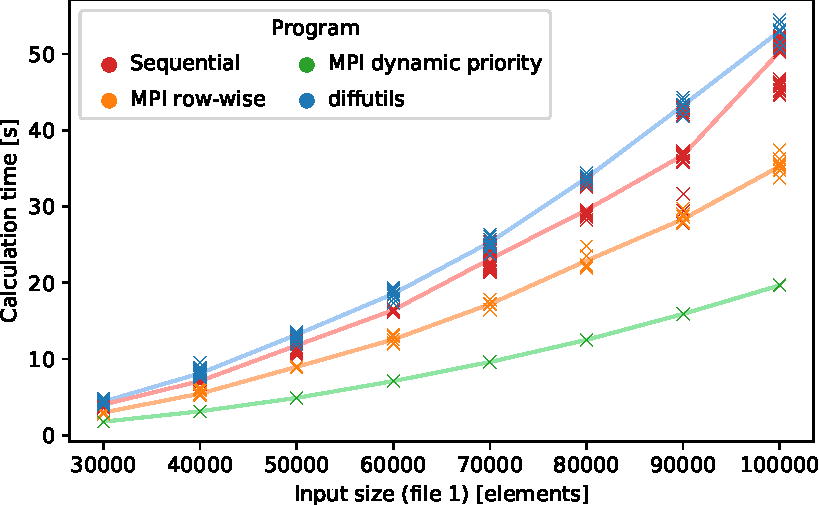
\includegraphics[width=\linewidth]{images/sequential-comparison.pdf}
  \caption{Calculation time of all algorithms when limited to a single process.}
  \label{results_sequential_comparison}
\end{figure}

To understand how our parallel algorithms scale, we ran them using various numbers of compute nodes. Figure \ref{results_scaling_time_mpi_row_wise} shows the calculation times from these experiments for our MPI row-wise algorithm. Using more nodes leads to a significant performance improvement. The curves for runtime seem to have approximately the ideal shape (proportional to $1 / \text{nodes}$). However it is not clear from this plot exactly how much less efficient the computation becomes as more nodes are used - that is investigated in a later plot. The runtime with DNA inputs shows the same trend as with synthetic inputs. For similar input sizes, the calculation time for DNA inputs is lower than for synthetic data, since they have a smaller edit distance.
% Unfortunately, the computing cluster was not available to run the large DNA input on all nodes, but we expect it to follow the same trend as the small DNA.

\begin{figure}[hbt]\centering
  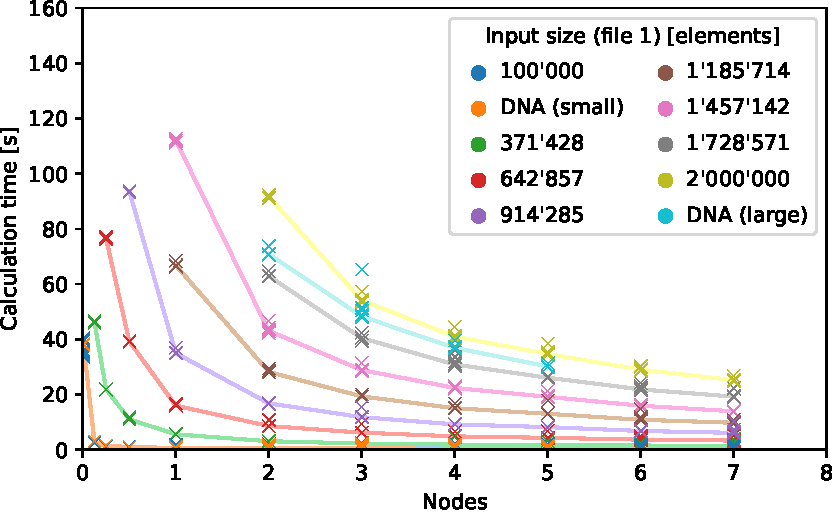
\includegraphics[width=\linewidth]{images/scaling-time-mpi-row-wise.pdf}
  \caption{Calculation time of the MPI row-wise algorithm with varying parallelism and input sizes.}
  \label{results_scaling_time_mpi_row_wise}
\end{figure}

Figure \ref{results_scaling_time_mpi_dynamic_priority} shows the results of an identical scaling experiment for our MPI dynamic priority algorithm. With one process the MPI dynamic priority algorithm is faster than MPI row-wise (as in figure \ref{results_sequential_comparison}). With half a node both algorithms have approximately the same speed. However the MPI dynamic priority algorithm becomes slower than the MPI row-wise algorithm once more nodes are used. This is surprising since the dynamic priority algorithm was designed to avoid blocking waits. We were not able to identify the cause of this bad scaling (which is difficult, since the behavior of the algorithm is very dynamic). Note that even with this inefficiency, using more nodes (for the number of nodes we tested) still reduces the total execution time. 

\begin{figure}[hbt]\centering
  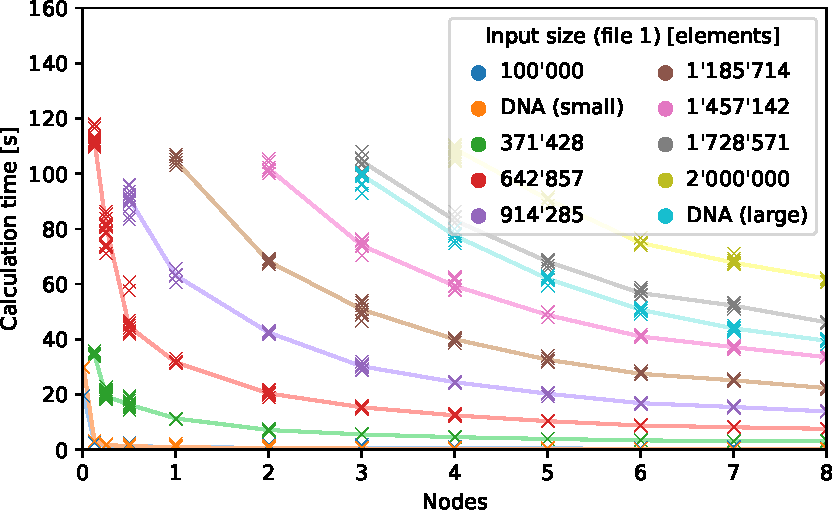
\includegraphics[width=\linewidth]{images/scaling-time-mpi-dynamic-priority.pdf}
  \caption{Calculation time of the MPI dynamic priority algorithm with varying parallelism and input sizes.}
  \label{results_scaling_time_mpi_dynamic_priority}
\end{figure}

To understand how efficiently our algorithms scale, we investigated the execution rate with a varying number of nodes (figure \ref{results_scaling_rate_mpi_row_wise}). We calculate rate as $\frac{n \cdot d}{t}$ which is the calculation time $t$ in seconds divided by the asymptotic runtime. For a fixed input (each curve in the plot), the rate is proportional to the speedup \cite{moreland2015formal} (which we do not calculate, since we do not have sequential measurements for large inputs). The dotted reference line approximates the rate that would be achieved with ideal linear speedup. This line is calculated based on the single run which achieves the highest rate with 1 node (for any input size). For the smallest input size (30'000 elements), the rate does not increase with more nodes. The overhead (e.g. MPI communication) likely dominates, since the total execution time (figure \ref{results_scaling_time_mpi_row_wise}) is very low. As inputs become larger, the row-wise algorithm becomes efficient. With the largest input sizes and number of nodes we tested, it scales nearly ideally.

\begin{figure}[hbt]\centering
  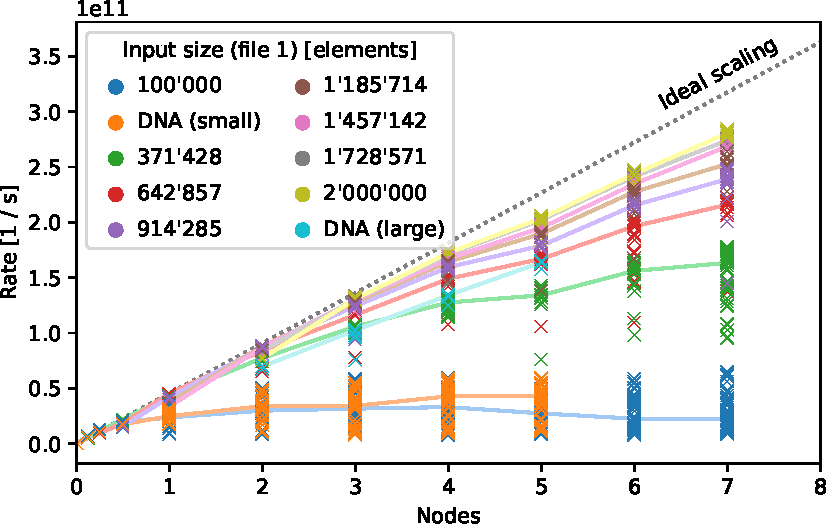
\includegraphics[width=\linewidth]{images/scaling-rate-mpi-row-wise.pdf}
  \caption{Rate of calculation (inverse runtime scaled by amount of work) of the MPI row-wise algorithm with varying parallelism and input sizes}
  \label{results_scaling_rate_mpi_row_wise}
\end{figure}

Figure \ref{results_scaling_rate_mpi_dynamic_priority} shows results in an identical format, but for our MPI dynamic priority algorithm. The MPI dynamic priority algorithm shows significantly worse than ideal scaling. Although the plotted curves for rate vs input size are roughly straight lines, the rate is not proportional to the number of nodes, as it would be for ideal scaling.

\begin{figure}[hbt]\centering
  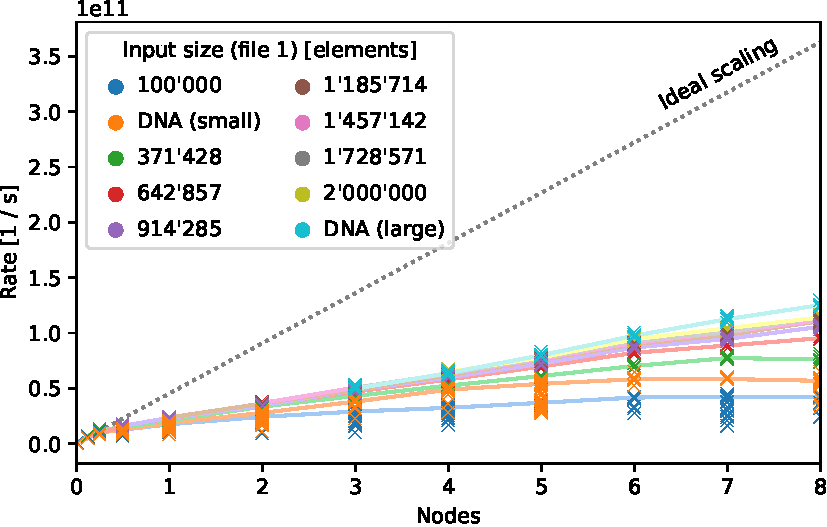
\includegraphics[width=\linewidth]{images/scaling-rate-mpi-dynamic-priority.pdf}
  \caption{Rate of calculation (inverse runtime scaled by amount of work) of the MPI dynamic priority algorithm with varying parallelism and input sizes}
  \label{results_scaling_rate_mpi_dynamic_priority}
\end{figure}

In all previously presented results, our algorithms had their SIMD features enabled (see ``Hardware \& software setup''). To investigate how this affects our algorithms, we repeated all the benchmarks from figures \ref{results_scaling_time_mpi_row_wise} and \ref{results_scaling_time_mpi_dynamic_priority} with the SIMD features disabled. Figure \ref{results_simd_comparison} shows the speedup from SIMD across those benchmarks. The speedup for each plotted point is calculated from the median runtime of each combination of algorithm, node count and input size. For the MPI row-wise algorithm, SIMD typically gives a speedup of 10\% - 30\%. Surprisingly enabling (the same) SIMD features in the MPI dynamic priority algorithm makes it run around 10\% slower. It is not clear what causes this slowdown. It may be necessary to investigate this together with the general scaling issues of the dynamic priority algorithm.

\begin{figure}[hbt]\centering
  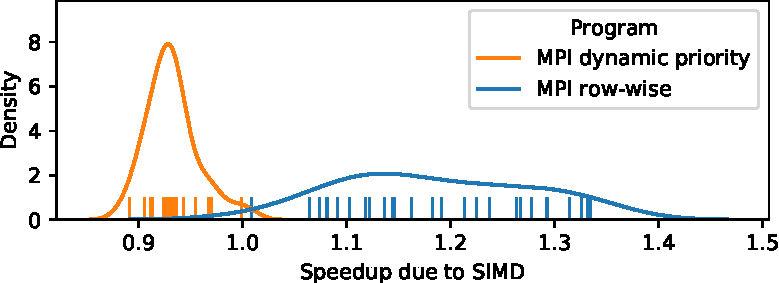
\includegraphics[width=\linewidth]{images/simd-comparison.pdf}
  \caption{Speedup (non-SIMD runtime / SIMD runtime) across all input sizes and node counts}
  \label{results_simd_comparison}
\end{figure}

% Next divide the experiments into classes, one paragraph for each. In each class of experiments you typically pursue one questions that then is answered by a suitable plot or plots. For example, first you may want to investigate the performance behavior with changing input size, then how your code compares to external benchmarks.
% 
% For some tips on benchmarking including how to create a decent viewgraph see pages 22--27 in Pueschel:10.

% {\bf Comments:}
% \begin{itemize}
% \item Create very readable, attractive plots (do 1 column, not 2 column plots
% for this report) with readable font size. However, the font size should also not be too large; typically it is smaller than the text font size.
% An example is in Fig.~\ref{fftperf} (of course you can have a different style).
% \item Every plot answers a question. You state this question and extract the
% answer from the plot in its discussion.
% \item Every plot should be referenced and discussed.
% \end{itemize}
% 
% \begin{figure}\centering
%   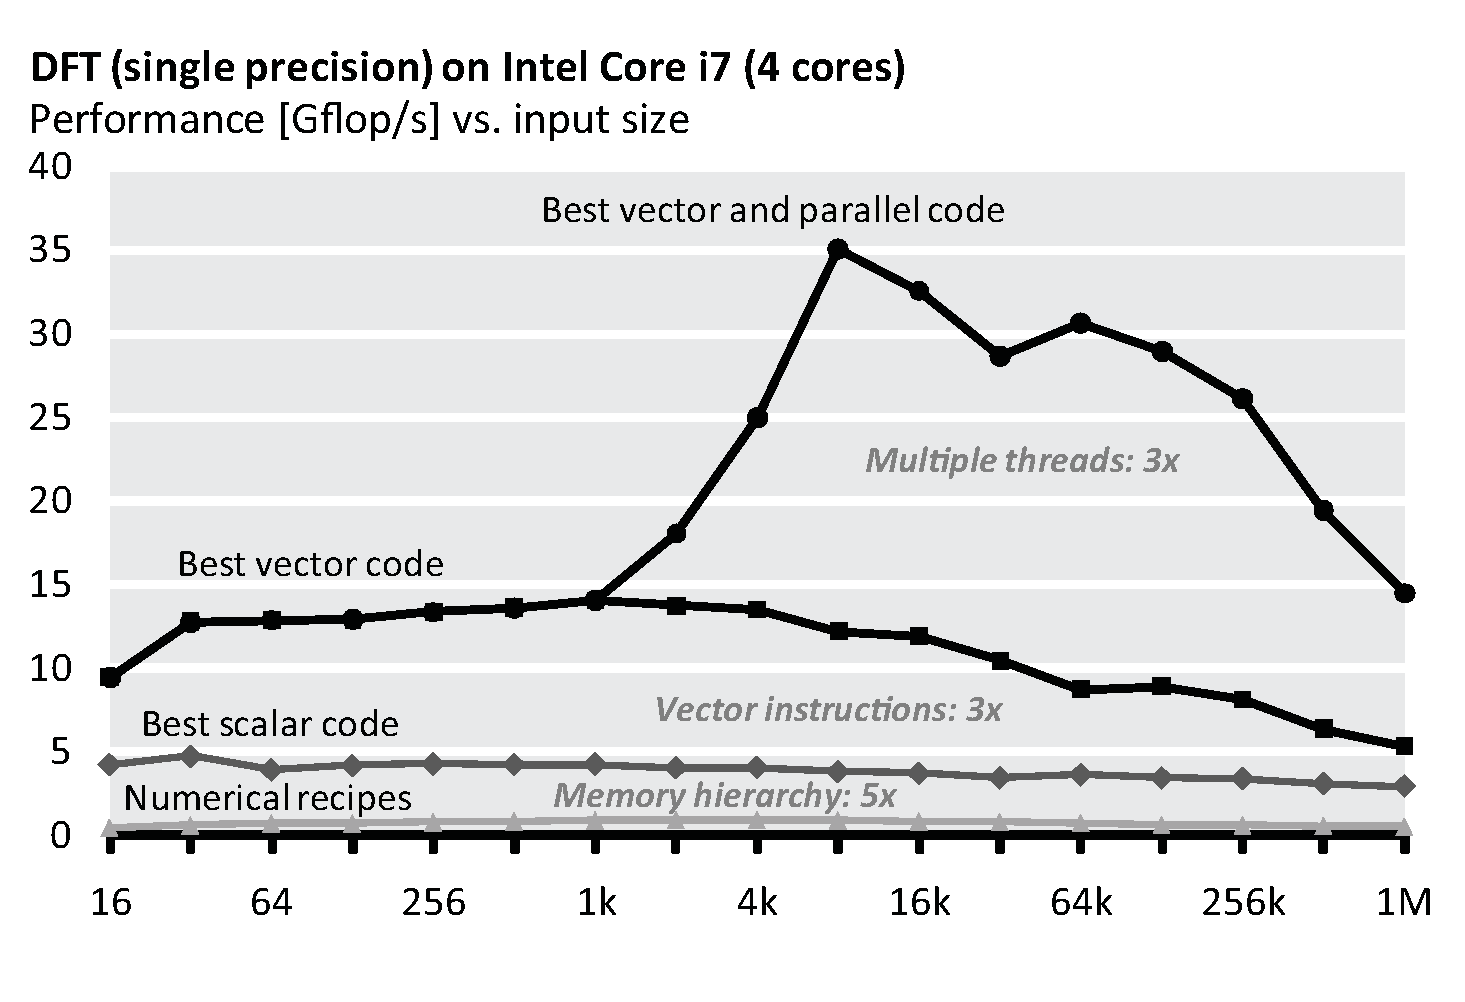
\includegraphics[scale=0.33]{dft-performance.eps}
%   \caption{Performance of four single precision implementations of the
%   discrete Fourier transform. The operations count is roughly the
%   same. The labels in this plot are maybe a little bit too small.\label{fftperf}}
% \end{figure}
